\documentclass{sig-alternate}
	\usepackage{algorithm}
	\usepackage{algpseudocode}
	\usepackage{listings}
	\usepackage{subfigure}

	\usepackage{tikz}
	\usepackage{tikz-uml}
	\tikzumlset{draw=black}
	\tikzumlset{fill class=white}
	\tikzumlset{fill template=white}
	\tikzumlset{fill package=white}

	\usepackage{pgf-umlsd}
	\usepgflibrary{arrows} % for pgf-umlsd

	\usepackage{bytefield}

	\usepackage{fourier}
	\usepackage{enumitem}

	\newcommand{\invitro}{\emph{in vitro} }
\begin{document}

\title{High-Level Sprout Geometry Extraction for In Vitro Angiogenesis Assays}
\numberofauthors{2}
\author{
	\alignauthor Gio Borje \\
		\affaddr{University of California, Irvine} \\
		\email{gborje@uci.edu}
	\alignauthor Craig Steinke \\
		\affaddr{University of California, Irvine} \\
		\email{csteinke@uci.edu}
}
\date{\today}
\maketitle

\begin{abstract}
	We have developed an automated image analysis system for the quantitative
	analysis of \invitro angiogenesis assays. Specifically, the system is
	designed for fibrin gel bead sprouting assays. The quantification system
	provides the number of primary sprouts, average branching factor and
	average length for each bead in an imaged assay.
\end{abstract}

\section{Introduction} % (fold)
\label{sec:Introduction}
	%% Motivation
	Angiogenesis is a mechanism for the formation of new blood vessels from
	pre-existing vessels. Additionally, angiogenesis is part of a critical
	phase in of solid tumor growth and metastasis. For solid tumors, the
	avascular growth phase enables an approximate maximum size of 1--2mm in
	diameter; on the other hand, the vascular growth phase enables unyielding
	tumor expansion and metastasis \cite{kerbel99}. Subsequently, \invitro
	angiogenesis assays are used to assess the impact of pro-angiogenic and
	antiangiogenic agents.

	%% Reference the Hughes Lab FBGSA
	The fibrin bead assay, developed by the Hughes Lab, begins by culturing
	endothelial cells as a monolayer on dextran-coated Cytodex beads. The
	beads are embedded into fibrin gels. In particular, human umbilical vein
	endothelial cells (HUVEC) are used. This method induces HUVEC to
	recapitulate multicellular capillaries in fibrin gels. Furthermore, the
	method for HUVEC promotes sprouting, lumen formation and long-term
	stability of neovessels. The high-resolution images of beads are then
	captured on an IX70 Olympus microscope \cite{nakatsu03}. A sample of such
	an image can be seen on Figure \ref{fig:monobead}.

	\begin{figure}[ht]
		\centering
		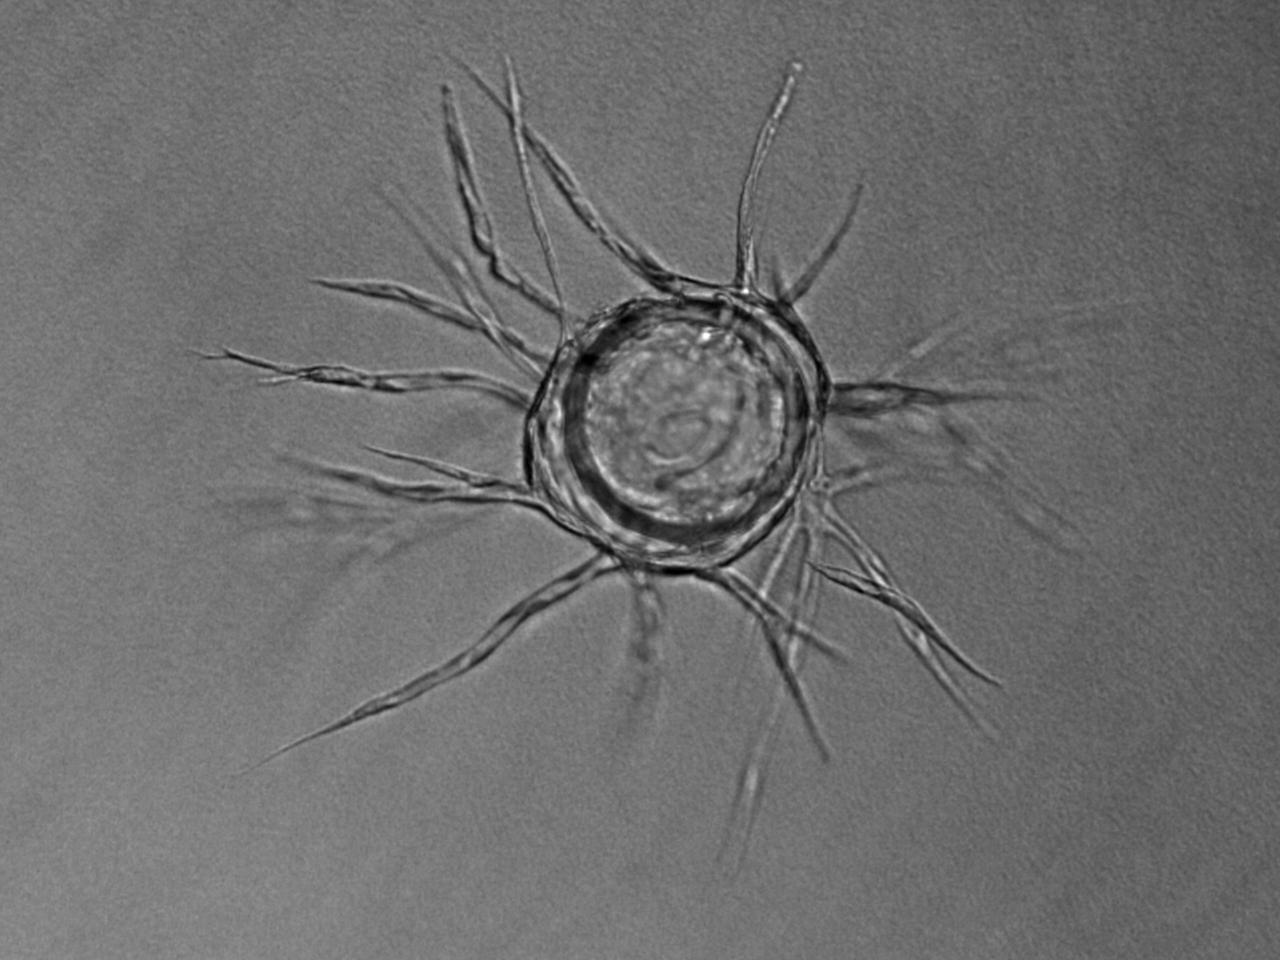
\includegraphics[width=6cm]{images/mono.jpg}
		\caption{Single Bead Image}
		\label{fig:monobead}
	\end{figure}

	%% How sprout counts were previously acquired
	Previously, the number of sprout counts per bead were measured by manual
	counting on the obtained images. Furthermore, the sprout length was
	measured in arbitrary units \cite{nakatsu03}. Our system relieves the
	laborious, manual analysis by quickly automating the detection and reliably
	analyzing of imaged assay features.

	The system, the High-Level Sprout Geometry (HLSG) Extractor, is designed to
	detect features, restore features and analyze the features of imaged
	assays. Features for detection include the Cytodex bead and its associated
	multicellular capillaries. However, due to the noise and depth of the image,
	the HLSG Extractor uses structural inpainting to restore and broken sprout
	features.

	In addition to the High-Level Sprout Geometry (HLSG) Extractor, a driver
	and report generator are implemented to drive functionality on sample
	images and generate reports on the analyses respectively.

	The following sections will proceed as follows. Section
	\ref{sec:Methodology} will describe an overview of the HLSG feature
	detection, feature restoration and analysis mechanisms. Section
	\ref{sec:Data Structures} will describe the data structures used to
	represent the HLSG and its properties. Section \ref{sec:System
	Architecture} shows how the system is designed for modularity and
	robustness.
% section Introduction (end)

\section{Methodology} % (fold)
\label{sec:Methodology}
	Our system enables feature set detection, minor feature restoration and
	quantitative analysis which can be decomposed into four stages. The
	first two stages detect feature sets: beads as features and then
	sprouts as features. In the third stage, the system attempts to restore
	a few sprout features by approximating and inpainting connections between
	broken sprout segments as well as filling holes. Finally, the system
	quantitatively analyzes the imaged assays through Sholl Analysis.

	\subsection{Bead Extraction} % (fold)
	\label{sub:Bead Extraction}
		\begin{figure}[htp!]
			\centering
			% \subfigure[Original]{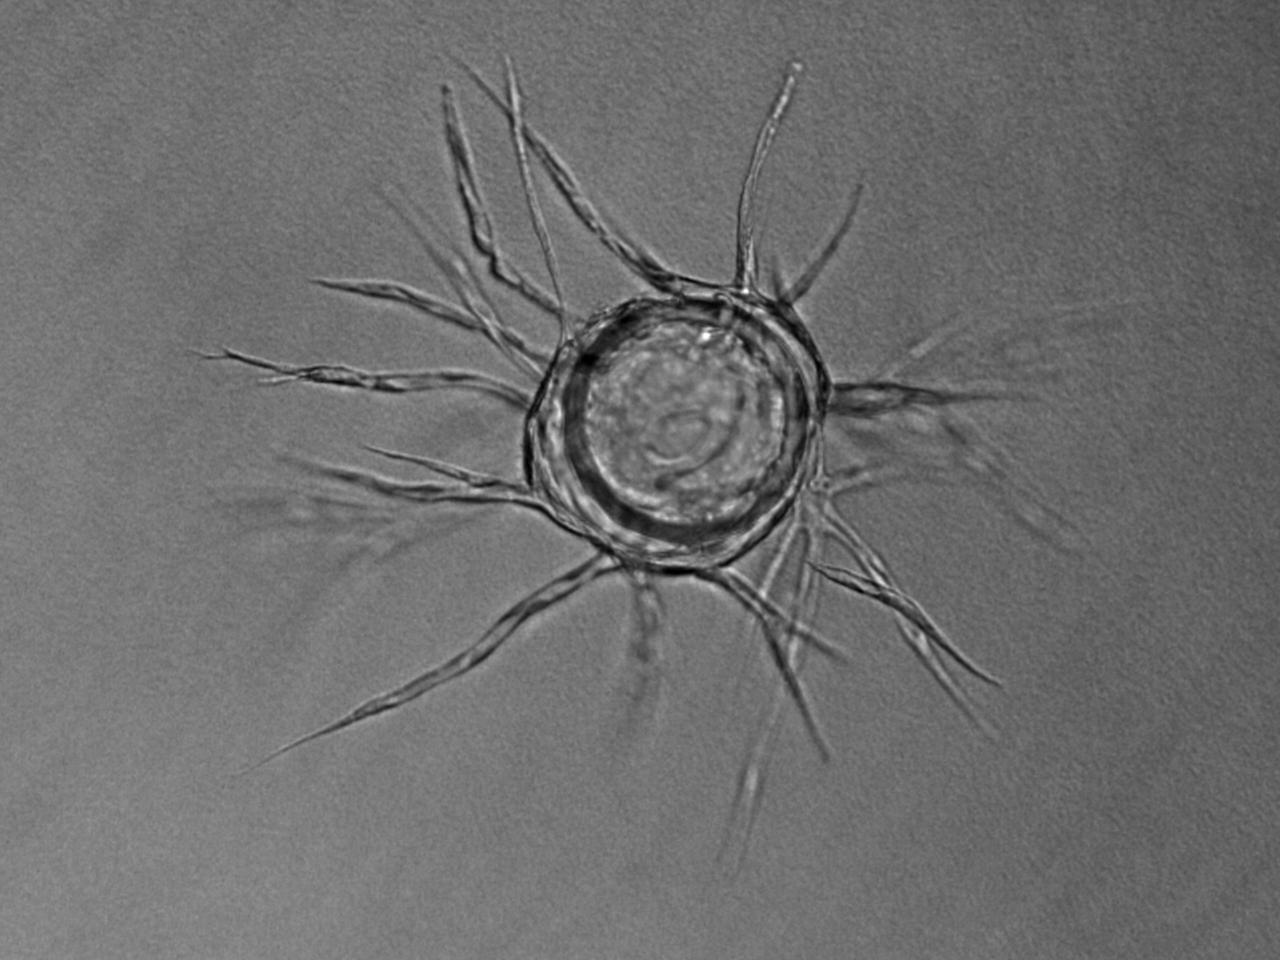
\includegraphics[width=4.1cm]{images/mono.jpg}}
			\subfigure[Edges]{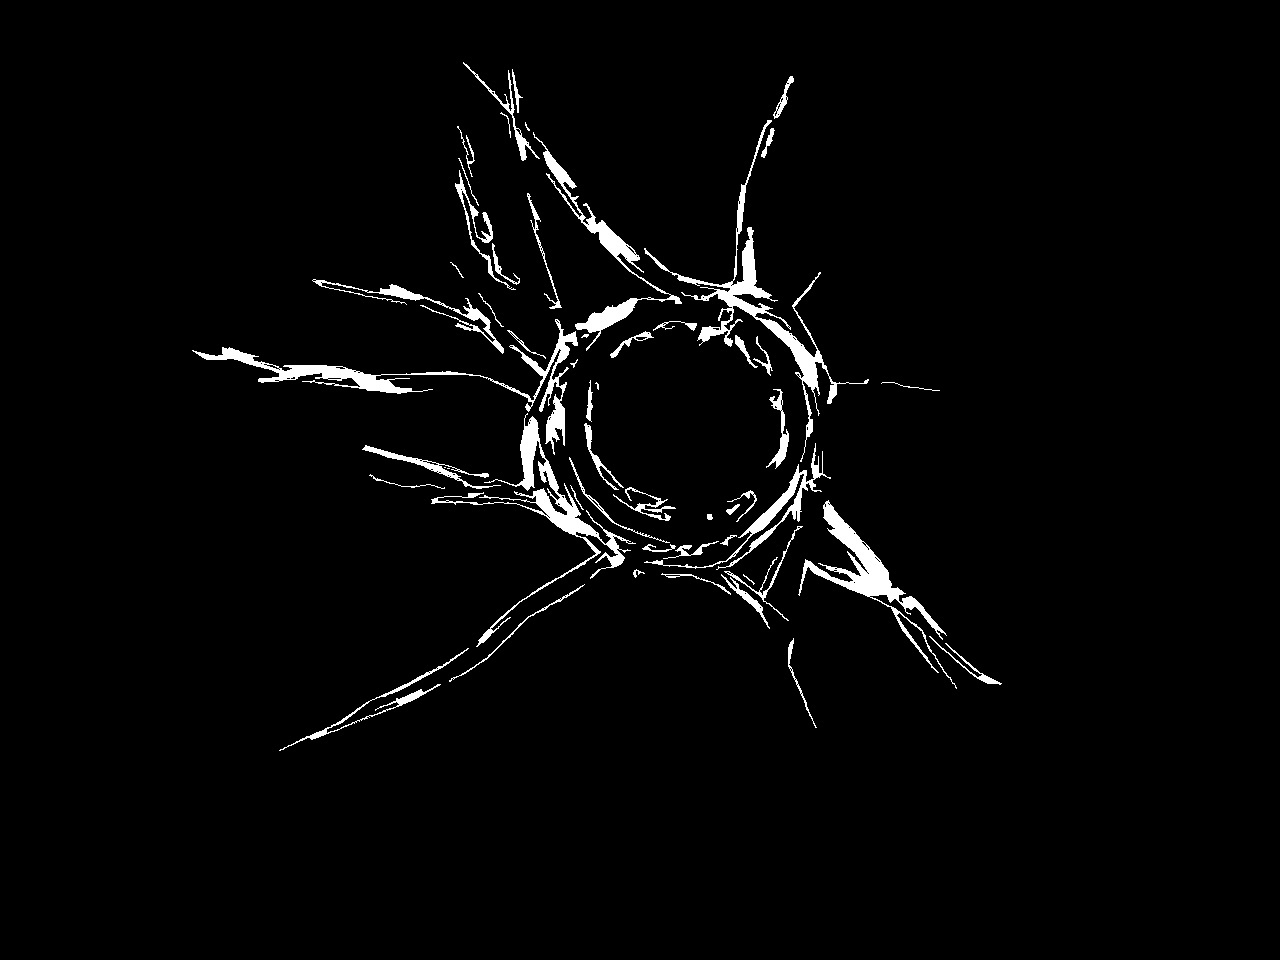
\includegraphics[width=4.1cm]{images/mono_preprocessed.jpg}}
			\subfigure[Bead Detection]{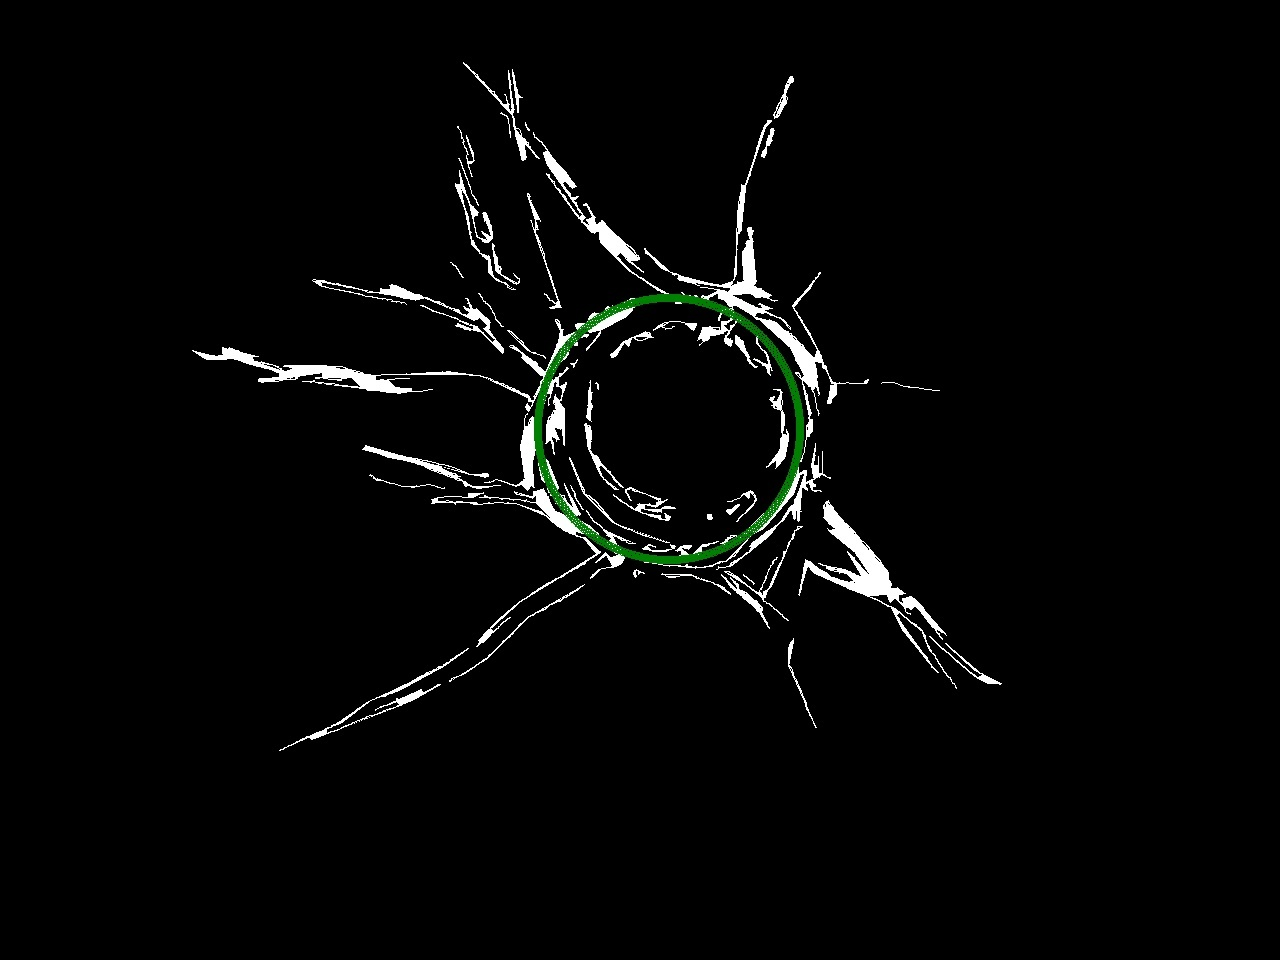
\includegraphics[width=4.1cm]{images/mono_found_circle.jpg}}
			\caption{Bead Extraction Outline}
			\label{fig:beadex}
		\end{figure}
		Bead extraction is a two-step process. To reduce noise, the system
		first smooths the image using a Gaussian blur. Second, circles in
		the image are detected using the circular Hough Transform. The
		circles detected correspond to the beads in the assay.
		Subsequently, the origin and radius of the bead is obtained.

		In order to avoid false bead detections, we enforce that the minimum
		distance between the origin of every pair of detected circles be four
		times the average bead radius i.e. each detected bead should at least
		be a bead apart.
	% subsection Bead Extraction (end)

	\subsection{Sprout Extraction} % (fold)
	\label{sub:Sprout Extraction}
		\begin{figure}[htp!]
			\centering
			\subfigure[Dilated]{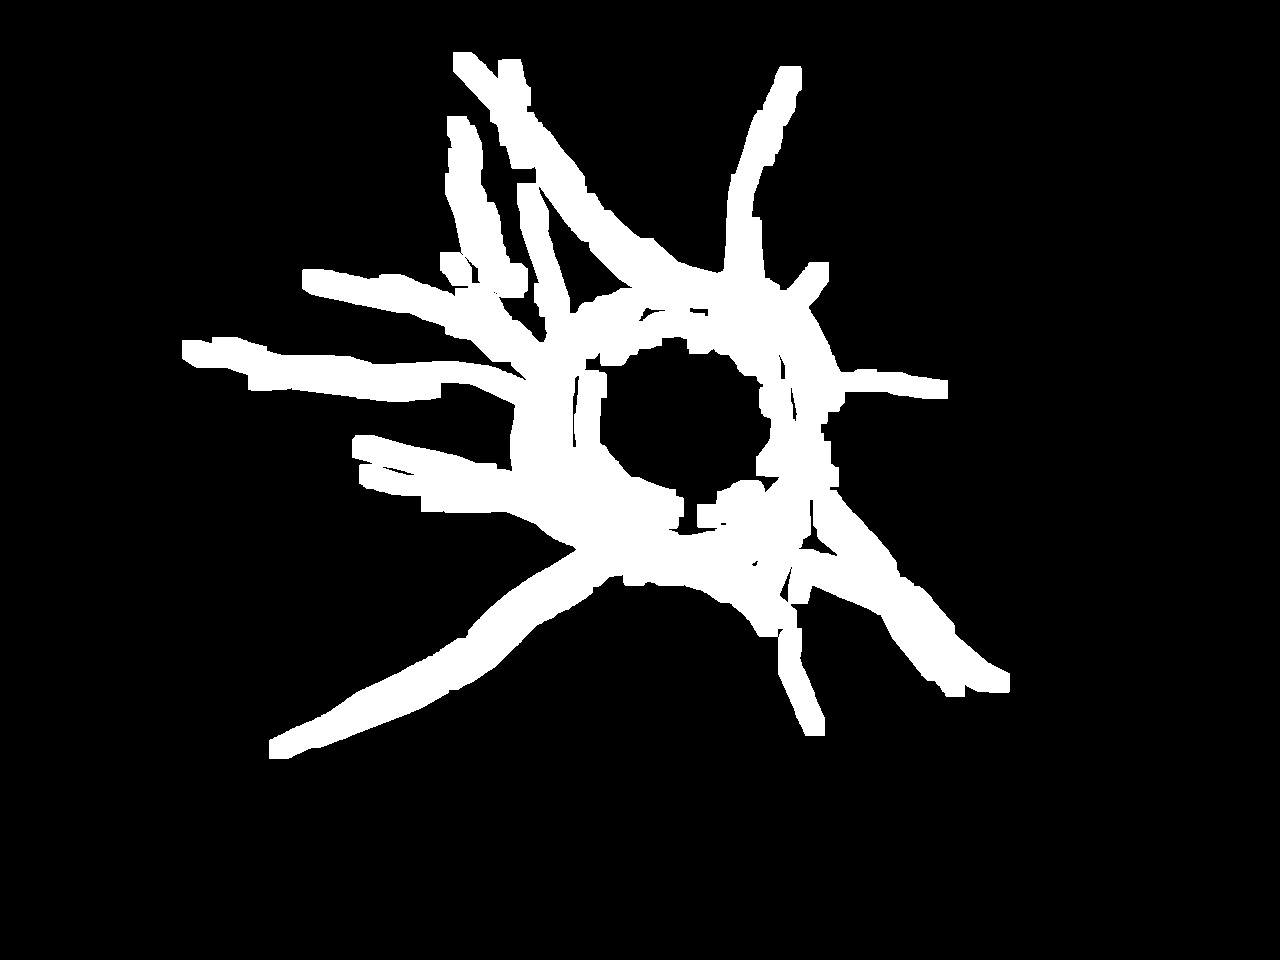
\includegraphics[width=4.1cm]{images/mono_dilated.jpg}}
			\subfigure[Skeleton]{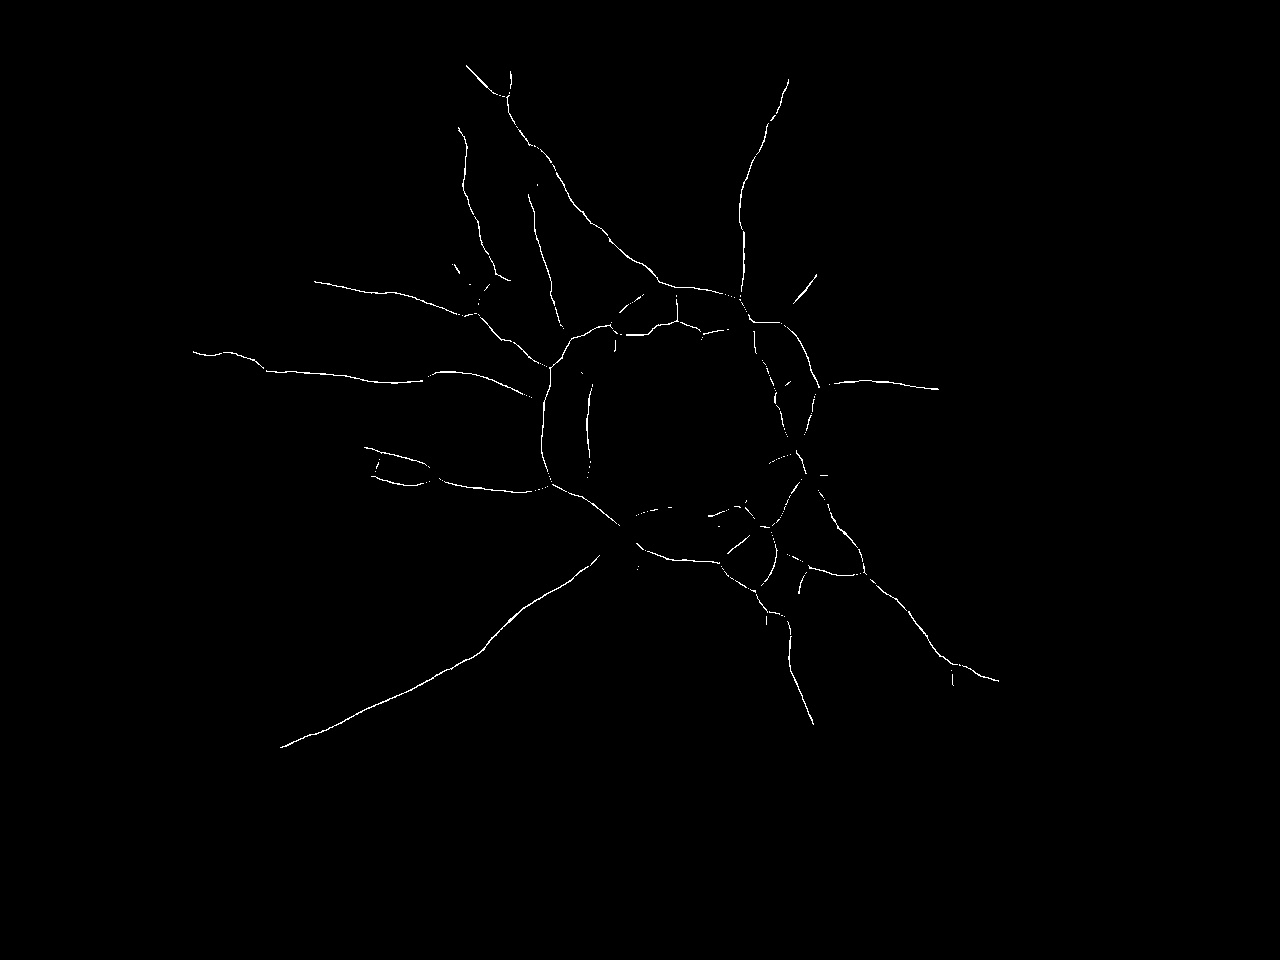
\includegraphics[width=4.1cm]{images/mono_skeletonized.jpg}}
			\caption{Sprout Extraction Outline}
			\label{fig:beadex}
		\end{figure}
		Sprout extraction depends on bead extraction because the beads must be
		masked before sprout extraction occurs to separate beads from sprouts.
		We mask the beads given the geometry of the circles. Due to the
		disconnectivity of sprouts in the assay, we begin by obtaining all
		sprout segments and represent them as line segments. We distinguish the
		end points of each line segment for connectivity. The start point, $S$,
		is the end point on the line segment such that it is closer to the
		origin of the line segment's closest bead. The end point, $E$, is the
		end point on the line segment such that it is farther from the origin
		of the line segment's closest bead.

		To determine which line segments belong to the same sprout, we use
		Euclidean distance between their start and end points enforced by
		the constraint that the end point must by closer to the origin of
		its closest's bead than the target start point. For example, two
		line segments are part of the same sprout if the distance between
		the start an end points are within a specified distance parameter,
		$d$.
	% subsection Sprout Extraction (end)

	\subsection{Sprout Restoration} % (fold)
	\label{sub:Sprout Restoration}
		There are two primary sources of degradation that we have discovered in
		the imaged assays: disjoint sprout segments and false capillary lumen
		detections i.e. holes. We will discuss our approaches to both problems
		independently. 
		
		The disjoint sprout segments are caused by the three-dimensional nature
		of the sprouts moving in and out of focus of the microscope.
		
		False capillary lumen detections are artifacts of the Canny
		edge-detection algorithm. By the morphology of these structures, we
		simply find the contours which enclose small holes and perform
		inpainting by polygon approximation using the Ramer-Douglas-Peucker
		algorithm.
	% subsection Sprout Restoration (end)

	\subsection{Sholl Analysis} % (fold)
	\label{sub:Sholl Analysis}
		Sholl Analysis is a quantitative method for quantitatively analyzing
		morphological characteristics of neurons \cite{sholl53}. Briefly, Sholl
		Analysis consists of counting the number of foreground to background
		crossings given concentric circles of a parameterized radius.

		\begin{algorithm}[ht!]
			\caption{Sholl Analysis}
			\begin{algorithmic}
				\Procedure{Sholl Analysis}{image, origin, radius}
					\State minRadius $\gets$ radius
					\State maxRadius $\gets$ $\min\left\{\text{image.width - origin.x, image.height - origin.y}\right\}$
					\State maxRadius $\gets$ $\min\left\{\text{maxRadius, origin.x, origin.y}\right\}$
					\State crossings $\gets$ []
					\ForAll{r $\in$ $[\text{minRadius}, \text{maxRadius}]$}
						\State crossings[r] $\gets$ 0
						\ForAll{pixel $\in$ ConcentricCircle(origin, radius)}
							\If{crossing detected at pixel}
								\State crossings[r] $\gets$ crossings[r] + 1
							\EndIf
						\EndFor
					\EndFor
					\State \Return crossings
				\EndProcedure
			\end{algorithmic}
		\end{algorithm}
	% subsection Sholl Analysis (end)
% section Methodology (end)

\section{Data Structures} % (fold)
\label{sec:Data Structures}
	The following data structures are used to implement the HLSG Extractor.
	\begin{figure}[!ht]
		\centering
		\begin{tikzpicture}[scale=0.5]
\umlclass[x=0,y=0]{BeadFeature}{
	+ center : (uint, uint) \\
	+ radius : uint \\
	}{}
\umlclass[x=4.5,y=0]{SproutFeature}{
	+ centroid : (uint, uint) \\
	+ length : uint \\
	+ width : uint \\
	}{}
\umlclass[x=4.5,y=-3]{RadialSegment}{
	+ inner : (uint, uint) \\
	+ outer : (uint, uint) \\
	+ blob : Blob
	}{}
%% Relations
\umlaggreg{BeadFeature}{SproutFeature}
\umluniaggreg{SproutFeature}{RadialSegment}
\end{tikzpicture}

		\caption{HLSG Extractor Features Class Diagram}
		\label{fig:classdiag}
	\end{figure}

	\subsection{Bead Feature} % (fold)
	\label{sub:Bead Feature}
		A bead feature is an abstraction of the Cytodex bead coated with
		endothelial cells in the assay. The geometry of the bead is intuitively
		circular; subsequently the geometry can is described by the descriptor
		in Figure \ref{fig:classdiag}.
	% subsection Bead Feature (end)

	\subsection{Sprout Feature} % (fold)
	\label{sub:Sprout Feature}
		A sprout feature is an abstraction of the blood vessels that develop
		through angiogenesis from the designed bead. Subsequently, sprout
		feature extraction is dependent upon bead descriptors. The sprout is
		actually comprised of a set of pixel segments because of the
		possibility that a sprout is disconnected.
	% subsection Sprout Feature (end)

	\subsection{Radial Line Segment} % (fold)
	\label{sub:Radial Line Segment}
		Due to the disconnectivity of sprouts, individual sprout segments
		are represented by a radially defined line segment. That is, we
		distinguish the end points from its radial distance from the origin
		of its corresponding bead. Given a line segment, we say that and
		end point is the \emph{inner point} if it is radially closer than
		its complementary end point; otherwise, we call the end point the
		\emph{outer point}.

		In addition to the distinguishable end points, a radial line
		segment is a line fit onto a corresponding blob of pixels which can
		be considered a sprout segment.
	% subsection Radial Line Segment (end)

	\subsection{Driver} % (fold)
	\label{sub:Driver}
		The Driver is responsible for parsing input from the user and emulating
		the encoded actions as functions of the HLSG Extractor. That is, the
		Driver acts similar to a REPL (Read-Eval-Print-Loop) that reads input
		from the user, evaluates the input and prints the corresponding output
		in a loop.  The set of commands available to the user is outlined Table
		\ref{tab:commands}.
	% subsection Driver (end)
% section Data Structures (end)

\section{System Architecture} % (fold)
\label{sec:System Architecture}
	The system requires Python version 2.7x with the SimpleCV package. The
	architecture of the system is based on our methodology for
	quantitatively analyzing \invitro angiogenesis. The system, however,
	incorporates modules for driving batch processes as well as a
	Read-Eval-Print-Loop (REPL) for console interaction. Finally, a module
	incorporated for generating CSV reports of the analysis. The sequence
	diagram for the system components are shown in Figure
	\ref{fig:sysarch}.
	\begin{figure*}[ht!]
		\centering
		\centering
\begin{sequencediagram}
\newinst[1]{client}{User}{}
\newinst[1]{driver}{Driver}{}
\newinst[2]{ex}{Extractors}{}
\newinst[3]{anal}{Sholl Analysis}{}
\newinst[1]{reportgen}{Report Generator}{}

\begin{mess}{client}{images}{driver}{}
	\begin{sdblock}{Main Loop}{}
		\begin{call}{driver}{ExtractHLSGs(img)}{ex}{hlsg}
			\begin{callself}{ex}{ExtractBeads(img)}{beads}
			\end{callself}

			\begin{sdblock}{Sprout Loop}{}
				\begin{callself}{ex}{ExtractSprouts(img, bead)}{sprouts}
				\end{callself}
			\end{sdblock}
		\end{call}

		\begin{call}{driver}{Analyze(hlsg)}{anal}{analysis}
		\end{call}
	\end{sdblock}

	\begin{call}{driver}{GenerateReport(analyses)}{reportgen}{report}
	\end{call}
\end{mess}
\end{sequencediagram}

		\caption{High-Level Architecture}
		\label{fig:sysarch}
	\end{figure*}

	The REPL module controls the interaction between the user and the
	system. Commands available in the REPL are shown in Table
	\ref{tab:commands}.
	\begin{table}[h!]
		\begin{tabular}{| l | l | p{4cm} |}
			\hline
			\textbf{Command} & \textbf{Output} & \textbf{Description} \\\hline
			extract [file] & HLSG of file & Extracts the HLSG of the given file. \\\hline
			extract [files] & HLSG of files & Extacts the HLSGs of the given files. \\\hline
			exit & Goodbye & Exits the system. \\\hline
		\end{tabular}
		\caption{Commands}
		\label{tab:commands}
	\end{table}
% section System Architecture (end)

\section{Results} % (fold)
\label{sec:Results}
	Display a comparison table with human counts.
	\begin{table}[h!]
		\centering
		\begin{tabular}{| l | l |}
			\hline
			\textbf{Human Sprout Counts} & \textbf{HLSG Sprout Counts} \\\hline
			0 & 0 \\\hline
			0 & 0 \\\hline
			0 & 0 \\\hline
			0 & 0 \\\hline
		\end{tabular}
		\caption{Result Comparison}
		\label{tab:resultcomp}
	\end{table}
% section Results (end)

\section{Discussion} % (fold)
\label{sec:Discussion}

Although the methodology is similar to AngioQuant, our method operates on
two-ridge structures \cite{niemisto05}.

% section Discussion (end)

\bibliography{prelim}
\bibliographystyle{plain}

\appendix
\section{Pseudo Code} % (fold)
\label{sec:Pseudo Code}
	This section outlines the pseudo-code for the Driver and HLSGExtractor
	operations. 

	\subsection{Driver} % (fold)
	\label{sub:Driver}
		The following pseudo-code outlines the Driver which reads input from
		the user, evaluates the input as a command, prints the output as a
		consequence of executing the command and then repeats this sequence of
		operations.
		\begin{algorithm}[ht!]
			\caption{Driver}
			\begin{algorithmic}
				\Procedure{Driver}{}
					\State running $\gets$ True
					\While{running}
						\State input $\gets$ read\_input()
						\State command $\gets$ parse(input)
						\State output $\gets$ HLSGExtractor.execute(command)
						\State print(output)
					\EndWhile
				\EndProcedure
			\end{algorithmic}
		\end{algorithm}

		Note that the driver executes while the \lstinline$running$ flag is
		true. Consequently, the REPL is responsible for setting this flag
		false.
	% subsection Driver (end)

	\subsubsection{Sprout Extractor} % (fold)
	\label{ssub:Sprout Extractor}
		Given an imaged assay and a set of bead features, the algorithm
		proceeds by masking the beads from the image. Next, a segmentation
		strategy is used to separate individual sprouts from the collection
		of globally detected sprouts. Finally, the segmentation strategy
		yields the detected feature set of sprouts.
		\begin{algorithm}[ht!] \caption{Sprout Extraction}
			\begin{algorithmic}
				\Procedure{ExtractSprouts}{img, beads}
					\State maskedImg $\gets$ maskBeads(img, beads)
					\State strategy $\gets$ SegmentStrategy(maskedImg,beads)
					\State sprouts $\gets$ strategy.segment()
					\State \Return sprouts
				\EndProcedure
			\end{algorithmic}
		\end{algorithm}
	% subsubsection Sprout Extractor (end)

	\subsubsection{HLSG Extractor} % (fold)
	\label{ssub:HLSG Extractor}
		\begin{algorithm}[ht!]
			\caption{HLSG Extraction}
			\begin{algorithmic}
				\Procedure{ExtractHLSGs}{img}
					\State beads $\gets$ ExtractBeads(img)
					\State sprouts $\gets$ ExtractSprouts(img, beads)
					\State hlsgs $\gets$ MapSproutsToBeads(sprouts, beads)
					\State \Return hlsgs
				\EndProcedure
			\end{algorithmic}
		\end{algorithm}
	% subsubsection HLSG Extractor (end)
% section Pseudo Code (end)


\end{document}
